\section{การออกแบบส่วนการวิเคราะห์ ตรวจสอบ และแนะนำท่าทางของผู้ใช้}
ในการออกแบบส่วนการวิเคราะห์ ตรวจสอบ และแนะนำท่าทางของผู้ใช้ จะแสดงเป็นแผนภาพการทำงานระหว่างระบบต่าง ๆ ได้ดังนี้
\begin{figure}
    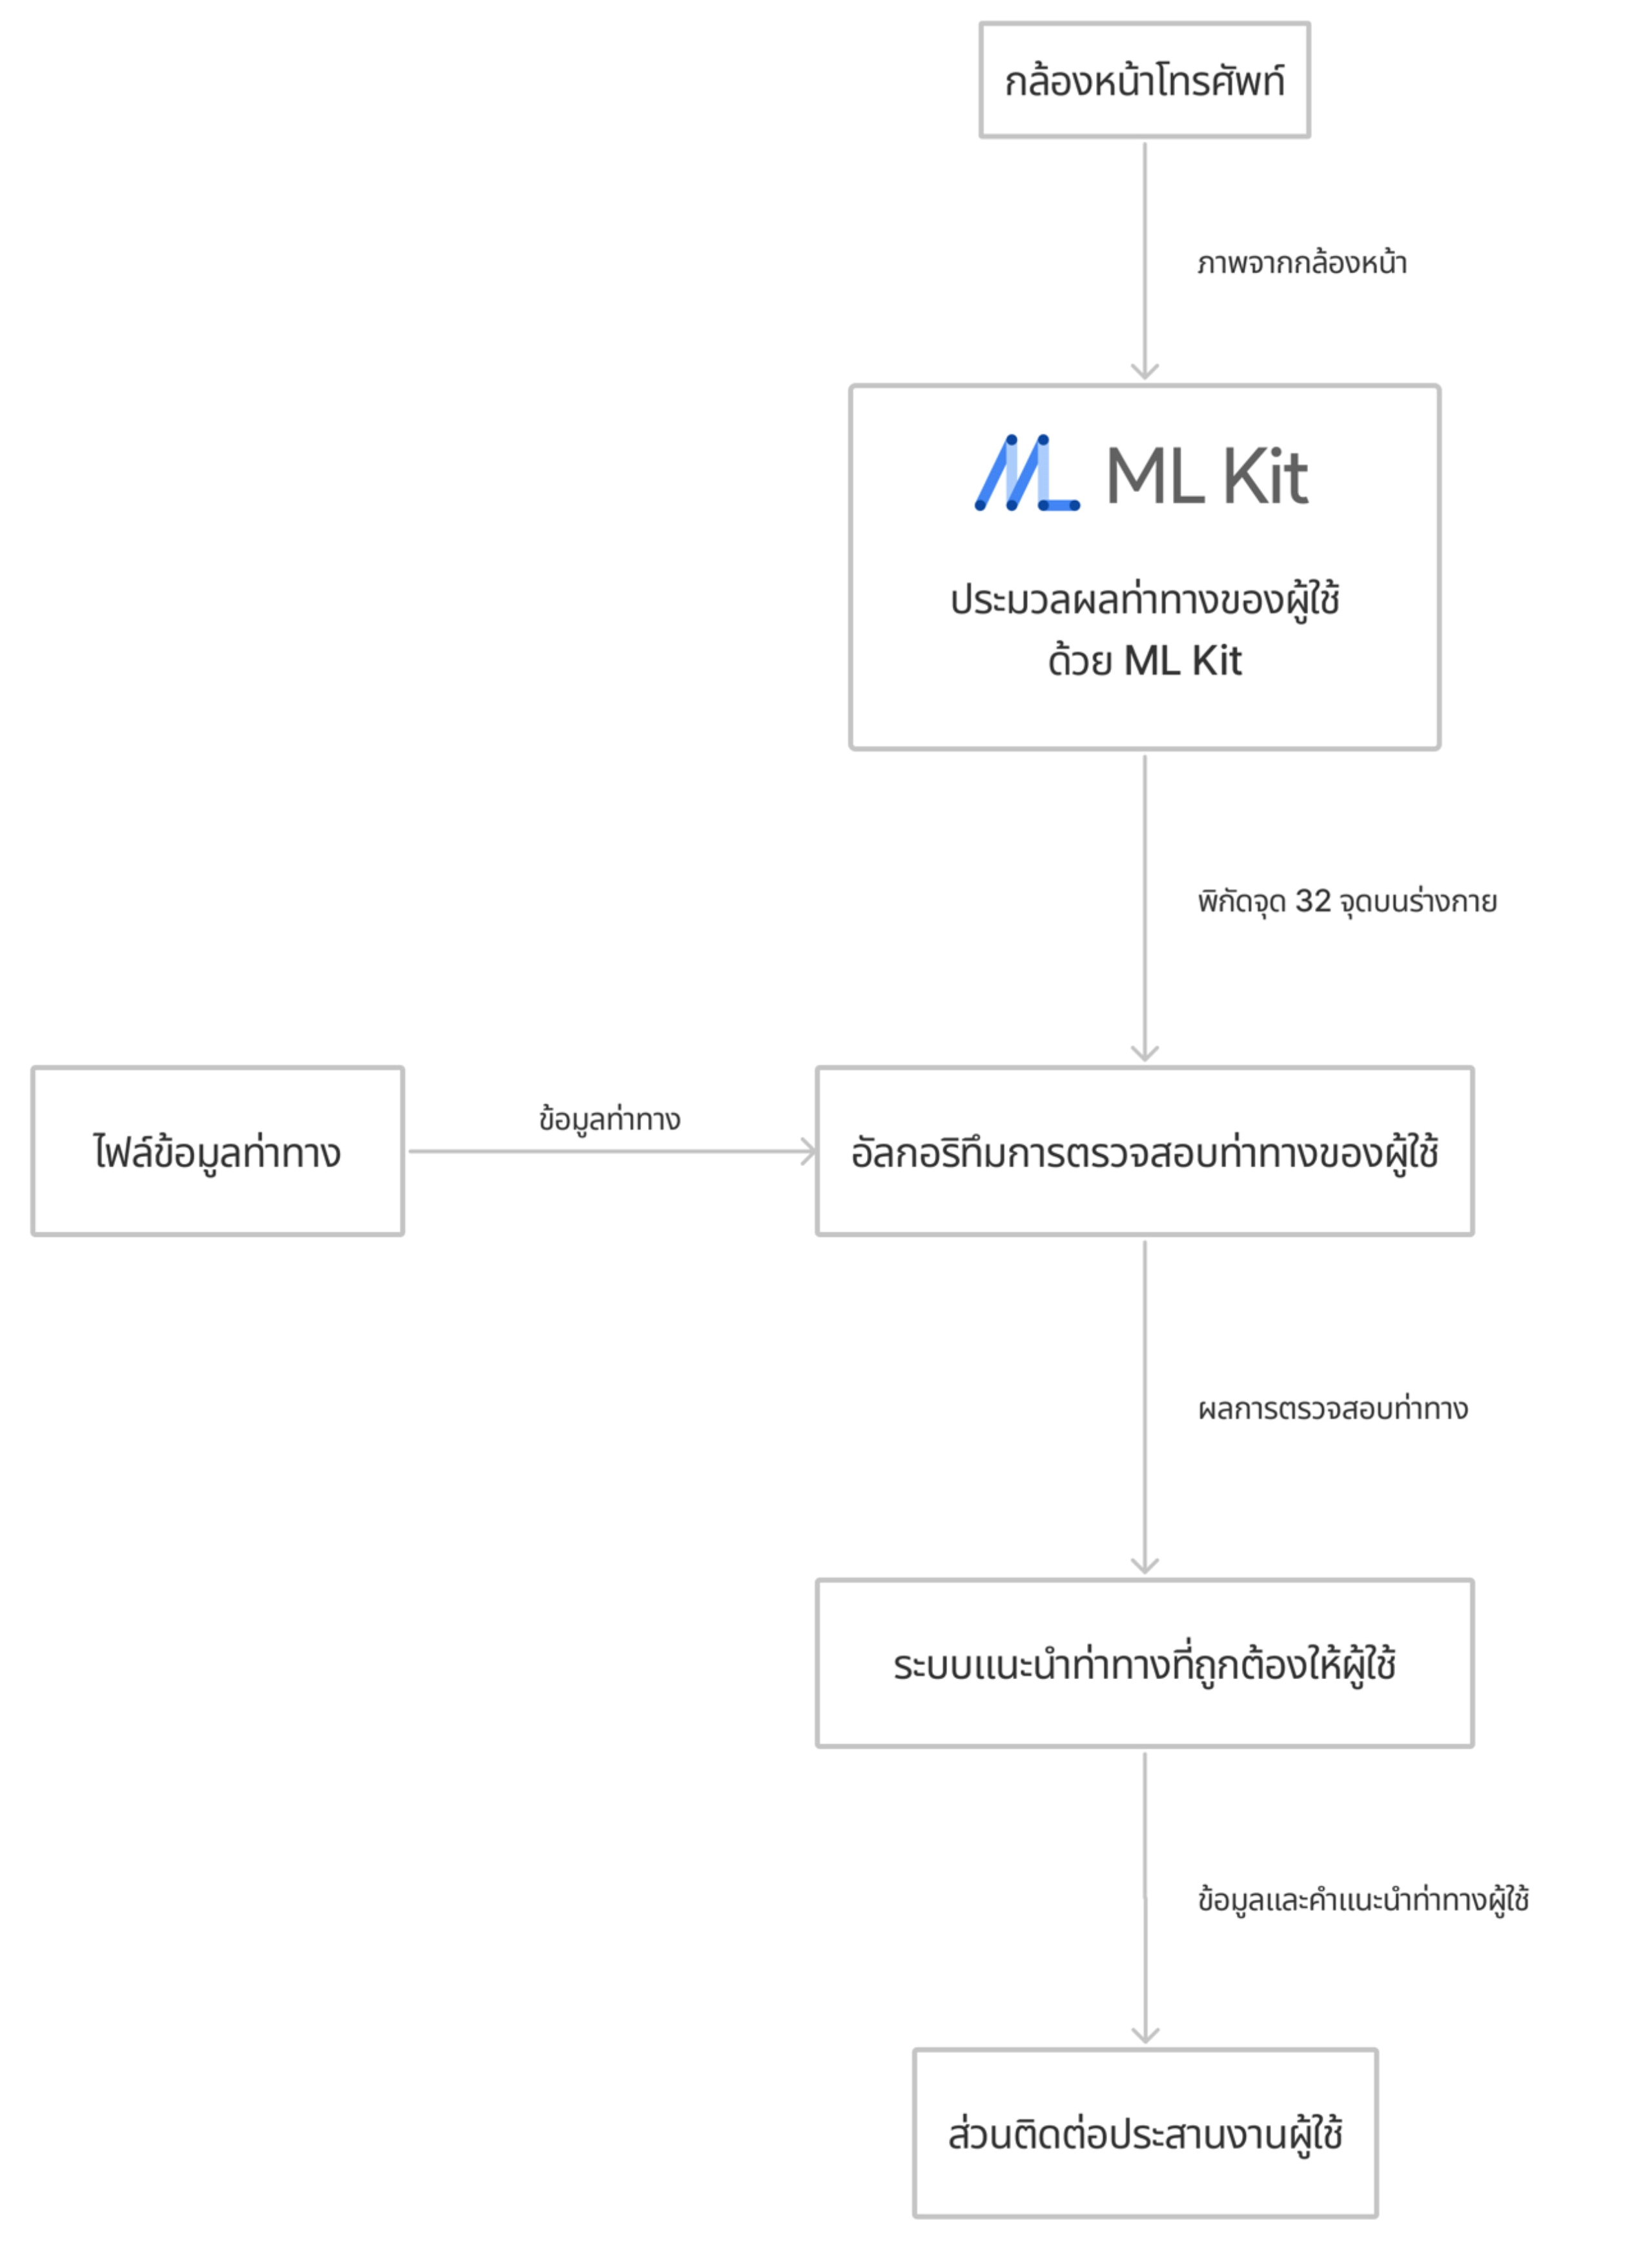
\includegraphics[width=\textwidth - 2cm]{chapter_3/pose overview2.jpg}
    \caption{ภาพรวมระบบการวิเคราะห์ ตรวจสอบ และแนะนำท่าทางของผู้ใช้}
\end{figure}
จากแผนภาพข้างต้น สามารถอธิบายออกเป็นส่วนต่าง ๆ ซึ่งจะแบ่งออกเป็น 4 ส่วน คือ ส่วนการประมวลผลท่าทางของผู้ใช้ด้วย ML Kit, ส่วนไฟล์ข้อมูลท่าทาง, ส่วนอัลกอริทึมการตรวจสอบท่าทางของผู้ใช้ และส่วนระบบแนะนำท่าทางที่ถูกต้องให้ผู้ใช้

\subsection{ส่วนการประมวลผลท่าทางของผู้ใช้ด้วย ML Kit}
สำหรับระบบการวิเคราะห์ท่าทาง จะใช้ API ของ ML Kit ในการตรวจจับท่าทางของผู้ใช้ ซึ่งจะได้พิกัดจุดทั้งหมด 32 จุดทั่วร่างกาย ซึ่งจะมีหน่วยเป็นพิกเซล
\begin{figure}
    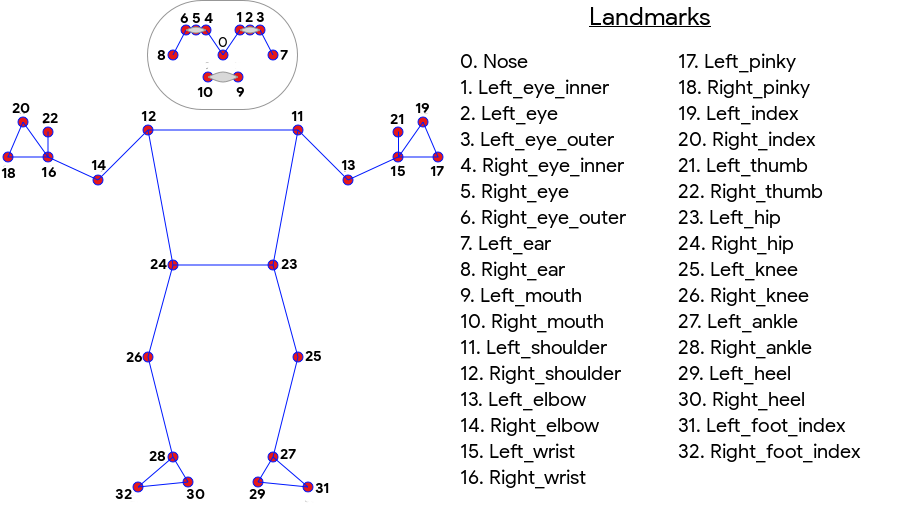
\includegraphics[width=\textwidth]{chapter_3/landmarks-fixed.png}
    \caption{แสดง Landmark จุดบนร่างกายที่ ML Kit สามารถตรวจจับได้}
\end{figure}

\subsection{ส่วนอัลกอริทึมการตรวจสอบท่าทางของผู้ใช้}
ในส่วนของการตรวจสอบท่าทางของผู้ใช้ ระบบจะนำข้อมูลพิกัดจุดที่ได้จากการประมวลผลในขั้นตอนที่แล้วมาใช้ โดยจะใช้ควบคู่กับไฟล์ข้อมูลท่าทางที่จะมีข้อมูลว่าจะต้องตรวจสอบท่าทางในจุดใดบ้าง ซึ่งจะประกอบไปด้วยคำสั่งที่จะให้ตรวจสอบ 2 คำสั่งคือ คำสั่งในการตรวจสอบองศาที่ทำมุมกันของจุดใด ๆ และคำสั่งตรวจสอบจุดใด ๆ ว่าอยู่ใกล้กันกับอีกจุดหนึ่งหรือไม่ โดยจะมีรายละเอียดในการหาผลลัพธ์ ดังนี้
\begin{enumerate}
    \item 	คำสั่งให้ตรวจสอบองศาของจุดที่ทำมุมกัน ในขั้นตอนแรกจะรับจุดทั้งหมด 3 จุด คือ จุด $A,B,C$ ซึ่งจะให้จุด $A$ เป็นจุดเริ่มต้น จากนั้นจึงคำนวณเวกเตอร์สามมิติซึ่งจะได้ออกมาเป็นเวกเตอร์ $\overrightarrow{AB}$ และ เวกเตอร์ $\overrightarrow{AC}$ ดังรูปภาพตัวอย่าง
    \begin{figure}
        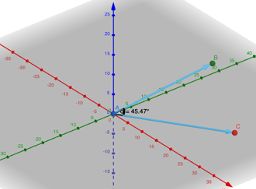
\includegraphics[width=7cm]{chapter_3/vector ex.png}
        \caption{แสดงตัวอย่างการหาเวกเตอร์ที่มีจุด A เป็นจุดร่วม}
    \end{figure}
    จากนั้นจึงหาองศาระหว่างเวกเตอร์ทั้งสองได้ จากสมการที่ \ref{eqn:vector}
    \begin{equation}
        \alpha = \arccos{\left( \frac{\overrightarrow{AB} \cdot \overrightarrow{AC}}{|\overrightarrow{AB}| \cdot |\overrightarrow{AC}|} \right)}
        \label{eqn:vector}
    \end{equation}
    และเมื่อได้องศาเรียบร้อยแล้ว จึงจะนำไปตรวจสอบกับค่าที่ได้รับว่าตรงตามที่ได้กำหนดไว้หรือไม่ ซึ่งจะแตกต่างกันตามที่ระบุไว้ในไฟล์ข้อมูลท่าทาง
    \item คำสั่งตรวจสอบจุดใด ๆ ว่าอยู่ใกล้กันกับอีกจุดหนึ่งหรือไม่ จะรับจุดจำนวน 2 จุด แล้วทำการคำนวณว่าจุดที่ได้รับ อยู่ใกล้เคียงกันหรือไม่ โดยการสร้างทรงกลมขึ้นมาโดยให้จุดที่ได้รับเป็นจุดศูนย์กลาง จะได้วงกลมขึ้นมาทั้งหมด 2 ลูกที่รัศมีเท่า ๆ กัน แล้วจึงทำการคำนวณว่าทรงกลมนี้มีการทับกันบางส่วนหรือทั้งหมดหรือไม่ โดยถ้ามีการทับกันจะถือว่าจุดทั้งสองอยู่ใกล้เคียงกัน
\end{enumerate}

\subsection{ส่วนไฟล์ข้อมูลท่าทาง}
ไฟล์ข้อมูลท่าทาง จะเป็นไฟล์ที่รวบรวมข้อมูลท่าทางทั้งหมดของทั้งคอร์ส ซึ่งภายในจะประกอบไปด้วยข้อมูลลำดับของท่าทาง, วิธีการนับท่าทางเป็นการจับเวลาหรือการนับการกระทำซ้ำ, ที่อยู่ของสื่อที่จะนำมาใช้สอนผู้ใช้ และเกณฑ์ต่าง ๆ ที่จะต้องตรวจสอบท่าทางนั้น ๆ และจะใช้ภาษา YAML ในการใช้งาน ซึ่งจะแสดงโครงสร้างไฟล์เป็น UML Class Diagram ได้ดังนี้

\begin{figure}
    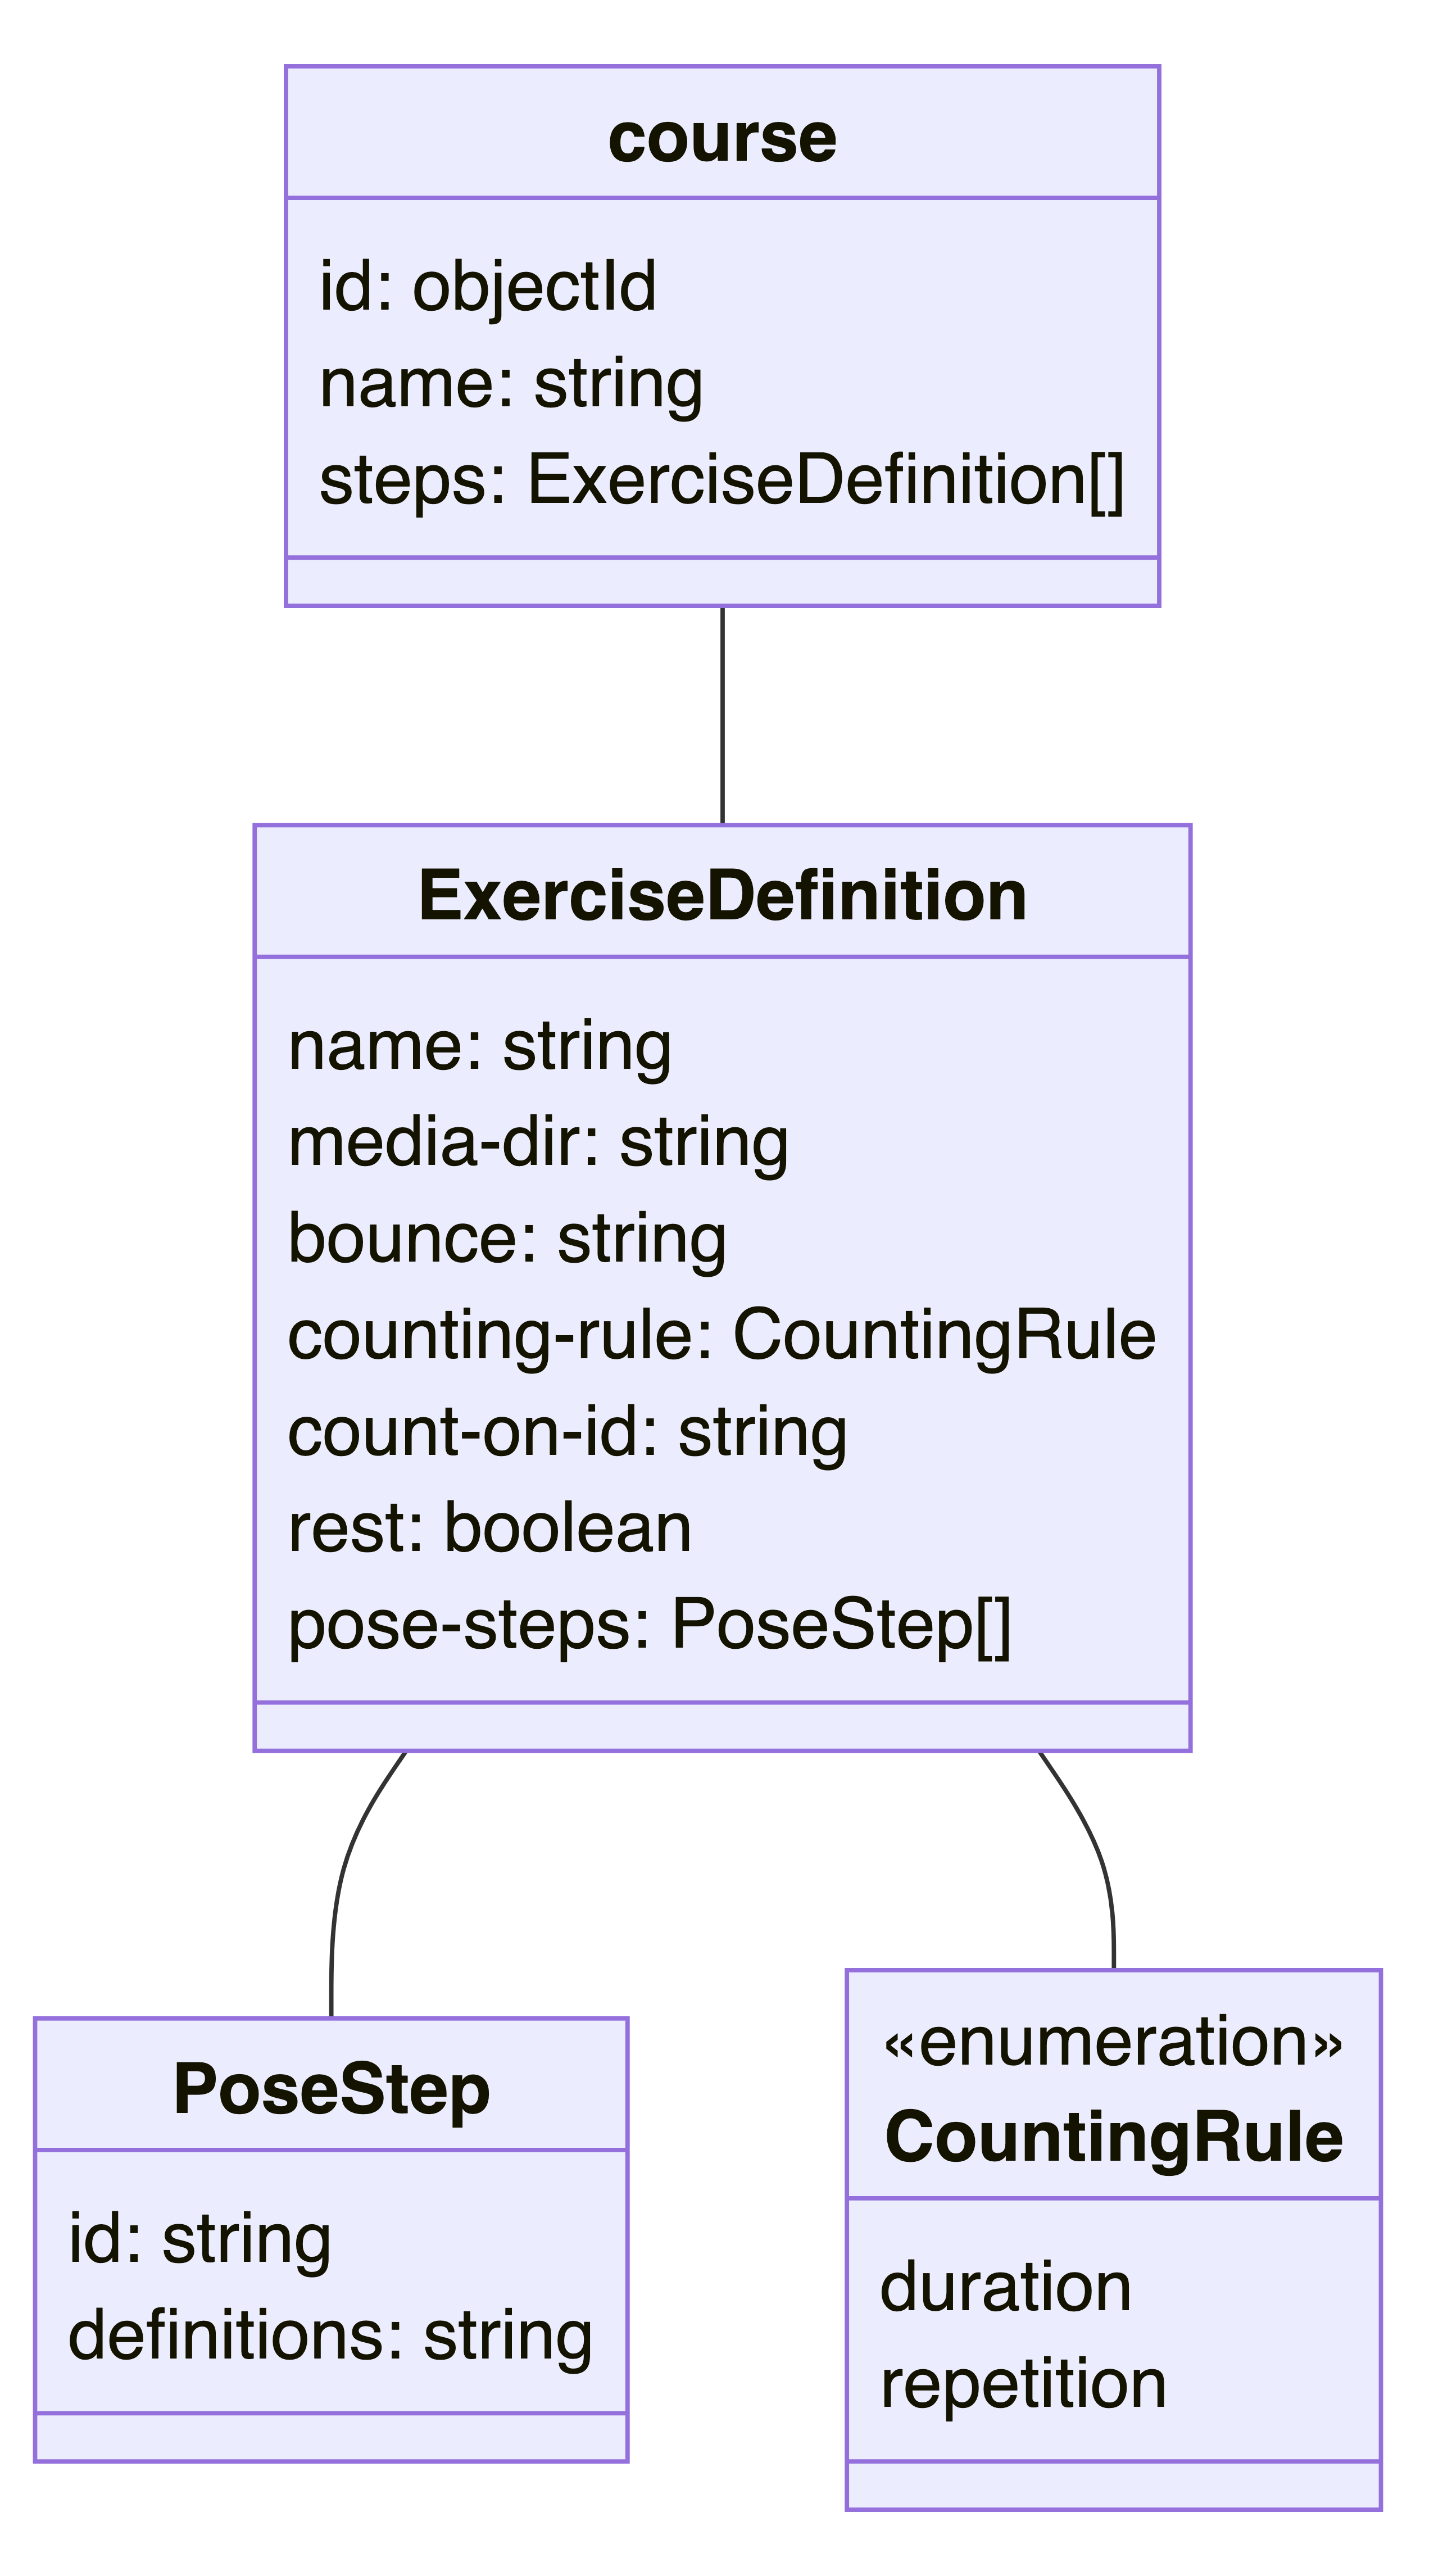
\includegraphics[width=\textwidth]{chapter_3/course-yaml-1.md.png}
    \caption{UML Class Diagram แสดงโครงสร้างไฟล์ข้อมูลท่าทาง}
\end{figure}
\clearpage
จากโครงสร้างไฟล์ จะมีรายละเอียดต่าง ๆ ในแต่ละคลาส ดังนี้
\begin{table}
    \caption{รายละเอียดฐานข้อมูลคลาส course}
    \begin{tabularx}{\textwidth}{ | l | l | X | }
        \hline
        \bf ชื่อคีย์			& \bf ชนิดตัวแปร       & \bf รายละเอียด    \\\hline
        id                  & objectId           & ID ของคอร์ส       \\\hline
        name                & string             & ชื่อคอร์ส            \\\hline
        steps               & ExerciseDefinition & อาเรย์ใช้ในการเก็บข้อมูลท่าทางการออกกำลังกายทั้งหมด รวมถึงลำดับของท่าทางของการออกกำลังกายในคอร์ส ซึ่งจะใช้เก็บข้อมูลของคลาส ExerciseDefinition \\\hline
    \end{tabularx}
\end{table}

ในคลาส ExerciseDefinition จะมีการเก็บท่าทางย่อยในคีย์ชื่อ poses ซึ่งในระบบจะมองว่าท่าทางการออกกำลังกายจะประกอบไปด้วยท่าทางย่อย ๆ ที่ต้องทำ เช่น ในการออกกำลังกายวิดพื้น จะมีท่าทางย่อย 2 ท่าทาง คือท่าทางเริ่มต้น และท่าทางเมื่องอศอก เป็นต้น โดยลำดับของท่าย่อย ๆ จะอ้างอิงตามลำดับในอาเรย์ ซึ่งถ้ามีการกำหนดให้ท่าทางนี้เป็นแบบไป-กลับ ระบบจะทราบว่าในท่าทางย่อย ๆ นี้เมื่อถึงท่าทางย่อยลำดับสุดท้ายแล้วผู้ใช้ต้องทำท่าทางย้อนกลับ ซึ่งจะมีรายละเอียด ดังนี้
\begin{table}
    \caption{รายละเอียดฐานข้อมูลคลาส ExerciseDefinition}
    \begin{tabularx}{\textwidth}{ | l | l | X | }
        \hline
        \bf ชื่อคีย์			& \bf ชนิดตัวแปร		& \bf รายละเอียด    \\\hline
        name                & string			& ชื่อท่าทาง           \\\hline
        mediaDir            & string			& ที่อยู่ URL ของสื่อที่จะนำมาใช้สอนผู้ใช้ \\\hline
        bounce              & boolean			& เป็นการกำหนดว่าท่าทางนี้เป็นแบบไป-กลับ หรือไม่ เช่น ในท่าทางวิดพื้นจะต้องมีการงอศอกลงและขึ้น ซึ่งจะต้องกำหนดให้เป็นท่าทางแบบไป-กลับ \\\hline
        criteria			& Criteria			& เกณฑ์ที่จะใช้ในการนับท่าทาง ซึ่งจะใช้การนับแบบจับเวลา หรือแบบการนับจำนวนครั้ง\\\hline
        posturePosition		& string			& ลักษณะของท่าทาง ซึ่งสามารถกำหนดให้เป็นแบบยืนหรือแบบนอน \\\hline
        cameraAngle			& string			& มุมกล้องที่จะใช้ถ่ายผู้ใช้ ซึ่งสามารถกำหนดให้เป็นแบบหน้าตรงและมุมข้างได้\\\hline
        facing				& string			& ในกรณีที่ลักษณะของท่าทางเป็นแบบนอน จะสามารถกำหนดได้ว่าจะต้องหันหน้าขึ้นหรือลง\\\hline
        poses				& Pose[]			& อาเรย์ที่ใช้อธิบายท่าทางย่อยในการออกกำลังกายนั้น ๆ\\\hline
        warningPose			& WarningPose[]		& อาเรย์ที่ใช้อธิบายท่าทางที่อาจจะทำให้ผู้ใช้บาดเจ็บได้\\\hline
    \end{tabularx}
\end{table}


\begin{table}
    \caption{รายละเอียดฐานข้อมูลคลาส Timer}
    \begin{tabularx}{\textwidth}{ | l | l | X | }
        \hline
        \bf ชื่อคีย์			& \bf ชนิดตัวแปร		& \bf รายละเอียด    \\\hline
        duration			& int				& ระยะเวลาที่จะใช้ หน่วยเป็นวินาที\\\hline
    \end{tabularx}
\end{table}

\begin{table}
    \caption{รายละเอียดฐานข้อมูลคลาส Counter}
    \begin{tabularx}{\textwidth}{ | l | l | X | }
        \hline
        \bf ชื่อคีย์			& \bf ชนิดตัวแปร		& \bf รายละเอียด    \\\hline
        countOnId			& string			& ID ของท่าทางที่เมื่อผู้ใช้ทำจะเป็นการนับ\\\hline
        repeat				& int				& จำนวนครั้งที่จะใช้ในการนับ \\\hline
    \end{tabularx}
\end{table}

\begin{table}
    \caption{รายละเอียดฐานข้อมูลคลาส Pose}
    \begin{tabularx}{\textwidth}{ | l | l | X | }
        \hline
        \bf ชื่อคีย์			& \bf ชนิดตัวแปร		& \bf รายละเอียด    \\\hline
        id					& string			& ชื่อท่าทาง           \\\hline
        definitions			& PoseDefinition	& เกณฑ์ต่าง ๆ ที่จะต้องตรวจสอบในท่าทางย่อย ๆ \\\hline
    \end{tabularx}
\end{table}

ในคีย์ definitions ในคลาส Pose จะสามารถกำหนดได้ว่าจะคำนวณโดยใช้การวัดองศา หรือการวัดว่าจุดได้แตะกันหรือไม่ ซึ่งจะมีรายละเอียด ดังนี้
\begin{table}
    \caption{รายละเอียดฐานข้อมูลคลาส Angle}
    \begin{tabularx}{\textwidth}{ | l | l | X | }
        \hline
        \bf ชื่อคีย์			& \bf ชนิดตัวแปร		& \bf รายละเอียด    \\\hline
        landmarks			& string[]			& อาเรย์ชื่อจุดบนร่างกายที่จะใช้ในการวัดองศา ซึ่งจะรับเข้ามา 2 landmarks โดยอ้างอิงชื่อ landmark จาก ML Kit\\\hline
        vertex				& string			& ชื่อจุดยอดที่จะใช้เป็นจุดที่จะวัดองศา\\\hline
        range				& int[]				& ช่วงองศาที่ถูกต้อง\\\hline
    \end{tabularx}
\end{table}

\begin{table}
    \caption{รายละเอียดฐานข้อมูลคลาส Touch}
    \begin{tabularx}{\textwidth}{ | l | l | X | }
        \hline
        \bf ชื่อคีย์			& \bf ชนิดตัวแปร		& \bf รายละเอียด    \\\hline
        landmarks			& string[]			& อาเรย์ชื่อจุดบนร่างกายที่จะใช้วัดว่าจุดได้แตะกันหรือไม่ โดยอ้างอิงชื่อ landmark จาก ML Kit\\\hline
    \end{tabularx}
\end{table}

จากองค์ประกอบของโครงสร้างไฟล์ข้อมูลท่าทางที่กล่าวมาข้างต้นทั้งหมด สามารถนำมาเขียนเป็นไฟล์ข้อมูลท่าทางในภาษา YAML ได้ดังตัวอย่างของท่าทางกระโดดตบ ซึ่งจะเป็นการนับจำนวนท่าทาง และท่าทาง Tree Pose ซึ่งจะเป็นการจับเวลาท่าทาง ดังต่อไปนี้
\begin{lstlisting}[caption=ตัวอย่างไฟล์ข้อมูลท่าทางของท่าทางกระโดดตบ (Jumping Jacks)]
id: courseId
name: Jumping Jacks
steps:
    - name: Jumping Jacks
    mediaDir: "https://storage.googleapis.com/fca-bucket/courses/jumping-jacks/jumping%20jacks.mp4"
    bounce: true
    criteria:
        counter:
        repeat: 5
        countOnId: cnt
    posturePosition: stand
    cameraAngle: front
    facing: up
    calculators:
        - name: right arm
        angle:
            landmarks: [ rightElbow, rightHip ]
            vertex: rightShoulder
        - name: left arm
        angle:
            landmarks: [ leftElbow, leftHip ]
            vertex: leftShoulder
        - name: clap
        touch:
            landmarks: [leftIndex, rightIndex]
    poses:
        - definitions:
            - calculator: right arm
            with:
                range: [ 0, 30 ]
            - calculator: left arm
            with:
                range: [ 0, 30 ]
            - calculator: clap
            with:
                touch: false
        - id: cnt
        definitions:
            - calculator: right arm
            with:
                range: [ 100, 180 ]
            - calculator: left arm
            with:
                range: [ 100, 180 ]
            - calculator: clap
            with:
                touch: true    
\end{lstlisting}
\begin{lstlisting}[caption=ตัวอย่างไฟล์ข้อมูลท่าทางของท่าทาง Tree Pose]
id: courseId
name: Tree Pose
steps:
  - name: Tree Pose Right Leg
    mediaDir: ""
    bounce: true
    criteria:
      timer:
        duration: 10
    posturePosition: stand
    cameraAngle: front
    facing: up
    calculators:
      - name: right arm
        angle:
          landmarks: [rightElbow, rightHip]
          vertex: rightShoulder
      - name: left arm
        angle:
          landmarks: [leftElbow, leftHip]
          vertex: leftShoulder
      - name: right leg
        angle:
          landmarks: [rightHip, rightAnkle]
          vertex: rightKnee
      - name: foot touch knee
        touch:
          landmarks: [rightFootIndex, leftKnee]

    poses:
      - definitions:
        - calculator: right arm
          with:
            range: [140,180]
        - calculator: left arm
          with:
            range: [140,180]
        - calculator: right leg
          with:
            range: [0,70]
        - calculator: foot touch knee
          with:
            touch: true
  - name: Tree Pose Left Leg
    mediaDir: ""
    bounce: true
    criteria:
      timer:
        duration: 10
    posturePosition: stand
    cameraAngle: front
    facing: up
    calculators:
      - name: right arm
        angle:
          landmarks: [rightElbow, rightHip]
          vertex: rightShoulder
      - name: left arm
        angle:
          landmarks: [leftElbow, leftHip]
          vertex: leftShoulder
      - name: left leg
        angle:
          landmarks: [leftHip, leftAnkle]
          vertex: leftKnee
      - name: foot touch knee
        touch:
          landmarks: [leftFootIndex, rightKnee]

    poses:
      - definitions:
        - calculator: right arm
          with:
            range: [140,180]
        - calculator: left arm
          with:
            range: [140,180]
        - calculator: left leg
          with:
            range: [0,70]
        - calculator: foot touch knee
          with:
            touch: true
\end{lstlisting}


\subsection{ส่วนการแนะนำท่าทางให้แก่ผู้ใช้}
เมื่อส่วนอัลกอริทึมการตรวจสอบท่าทางของผู้ใช้ ได้ประมวลผลท่าทางเรียบร้อยแล้ว ระบบจะส่งผลการตรวจสอบมายังส่วนการแนะนำท่าทางผู้ใช้ โดยจะทำการแปลงข้อมูลการตรวจสอบที่ได้ เป็นประโยคแนะนำท่าทางภาษาอังกฤษ เพื่อให้ผู้ใช้สามารถเข้าใจได้ง่าย และจะส่งผลลัพธ์การแนะนำท่าทางไปยังส่วนประสานงานผู้ใช้ เพื่อแสดงผลต่อไป